\documentclass{article}

\usepackage{graphicx}

\begin{document}



\begin{figure}[!ht]
  \centering
  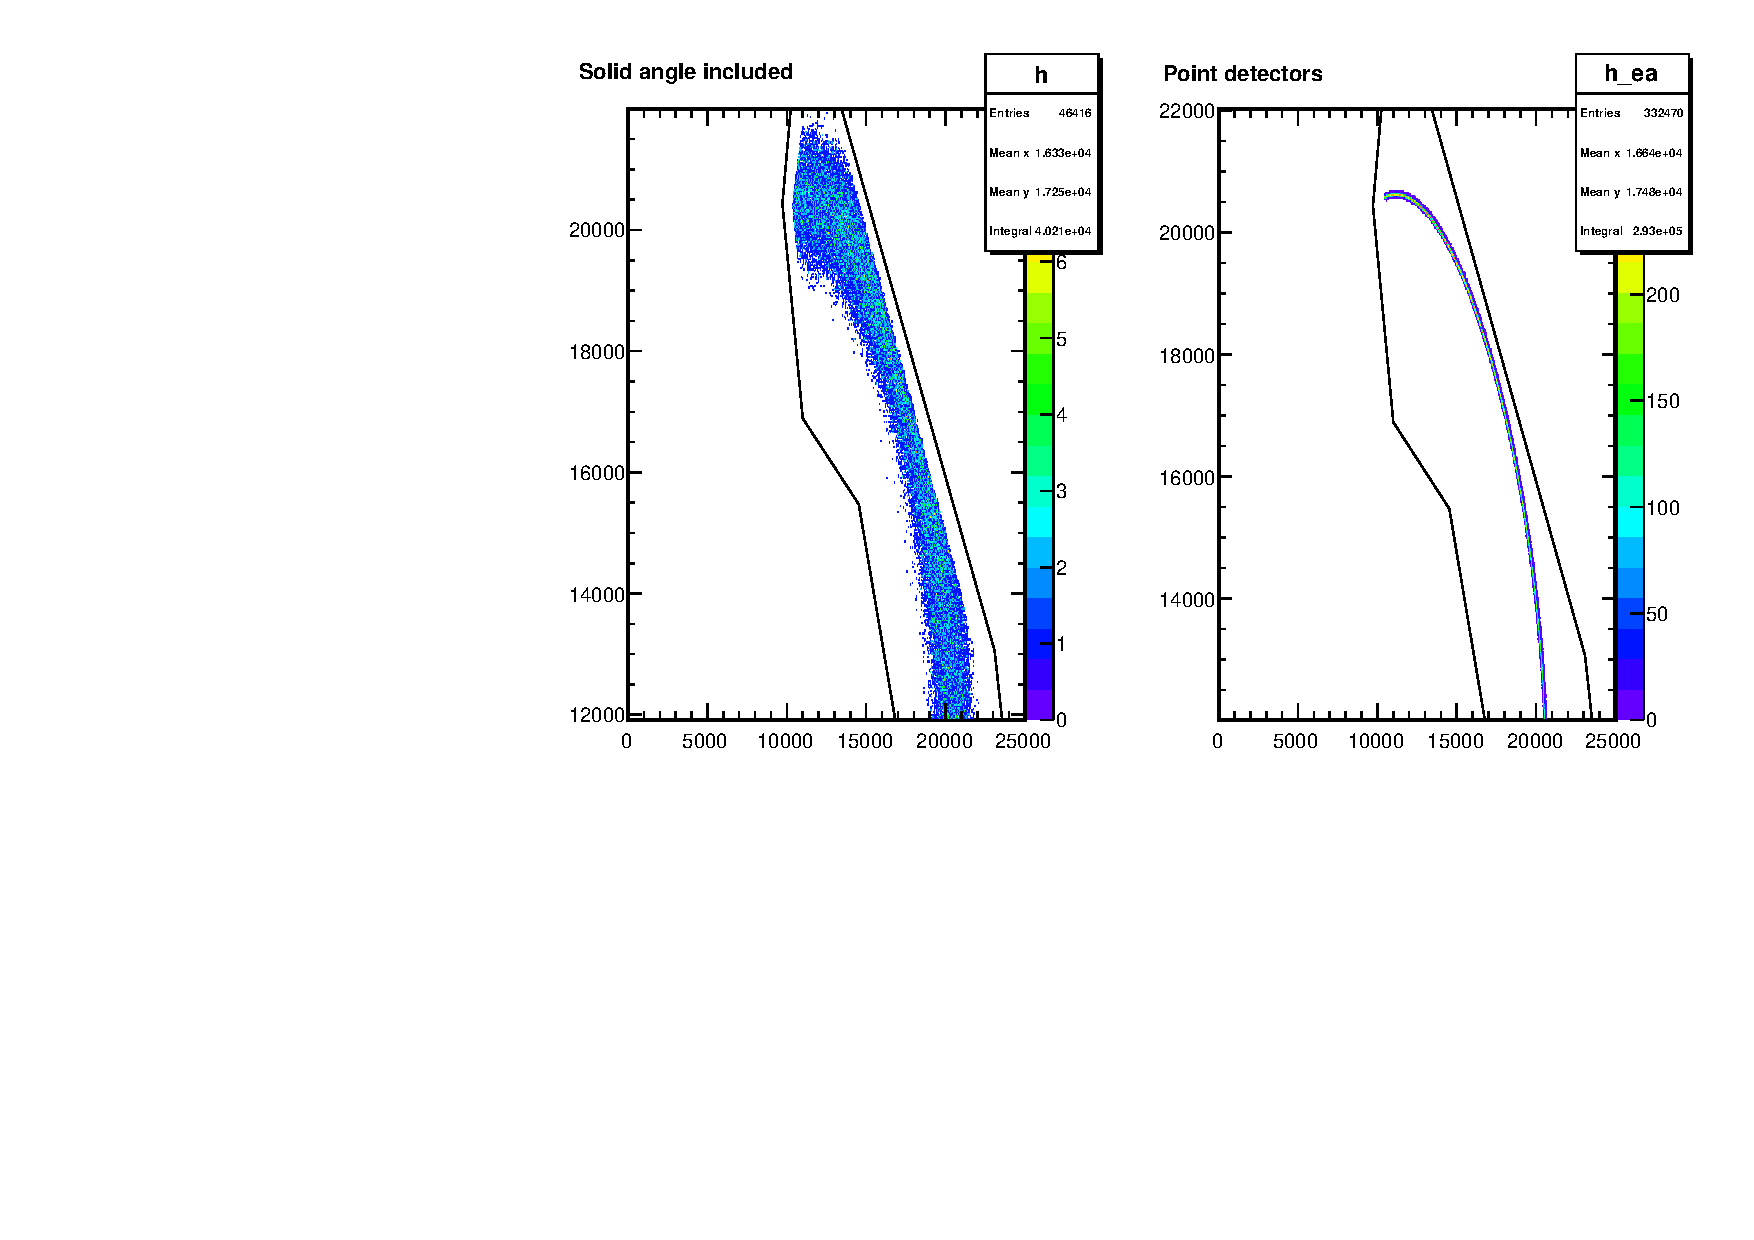
\includegraphics[width=\textwidth]{E1vsE2}
  \caption{2D E$_{\alpha 1}$ vs E$_{\alpha 2}$ plots for realistic
    collimators (on left) and ideal point detector and beam spots (on
    right). These are both cut spectra, and the axes should correspond
    roughly to the splitpole setup. }
  \label{fig:2D}
\end{figure}

\begin{figure}[!h]
  \centering
  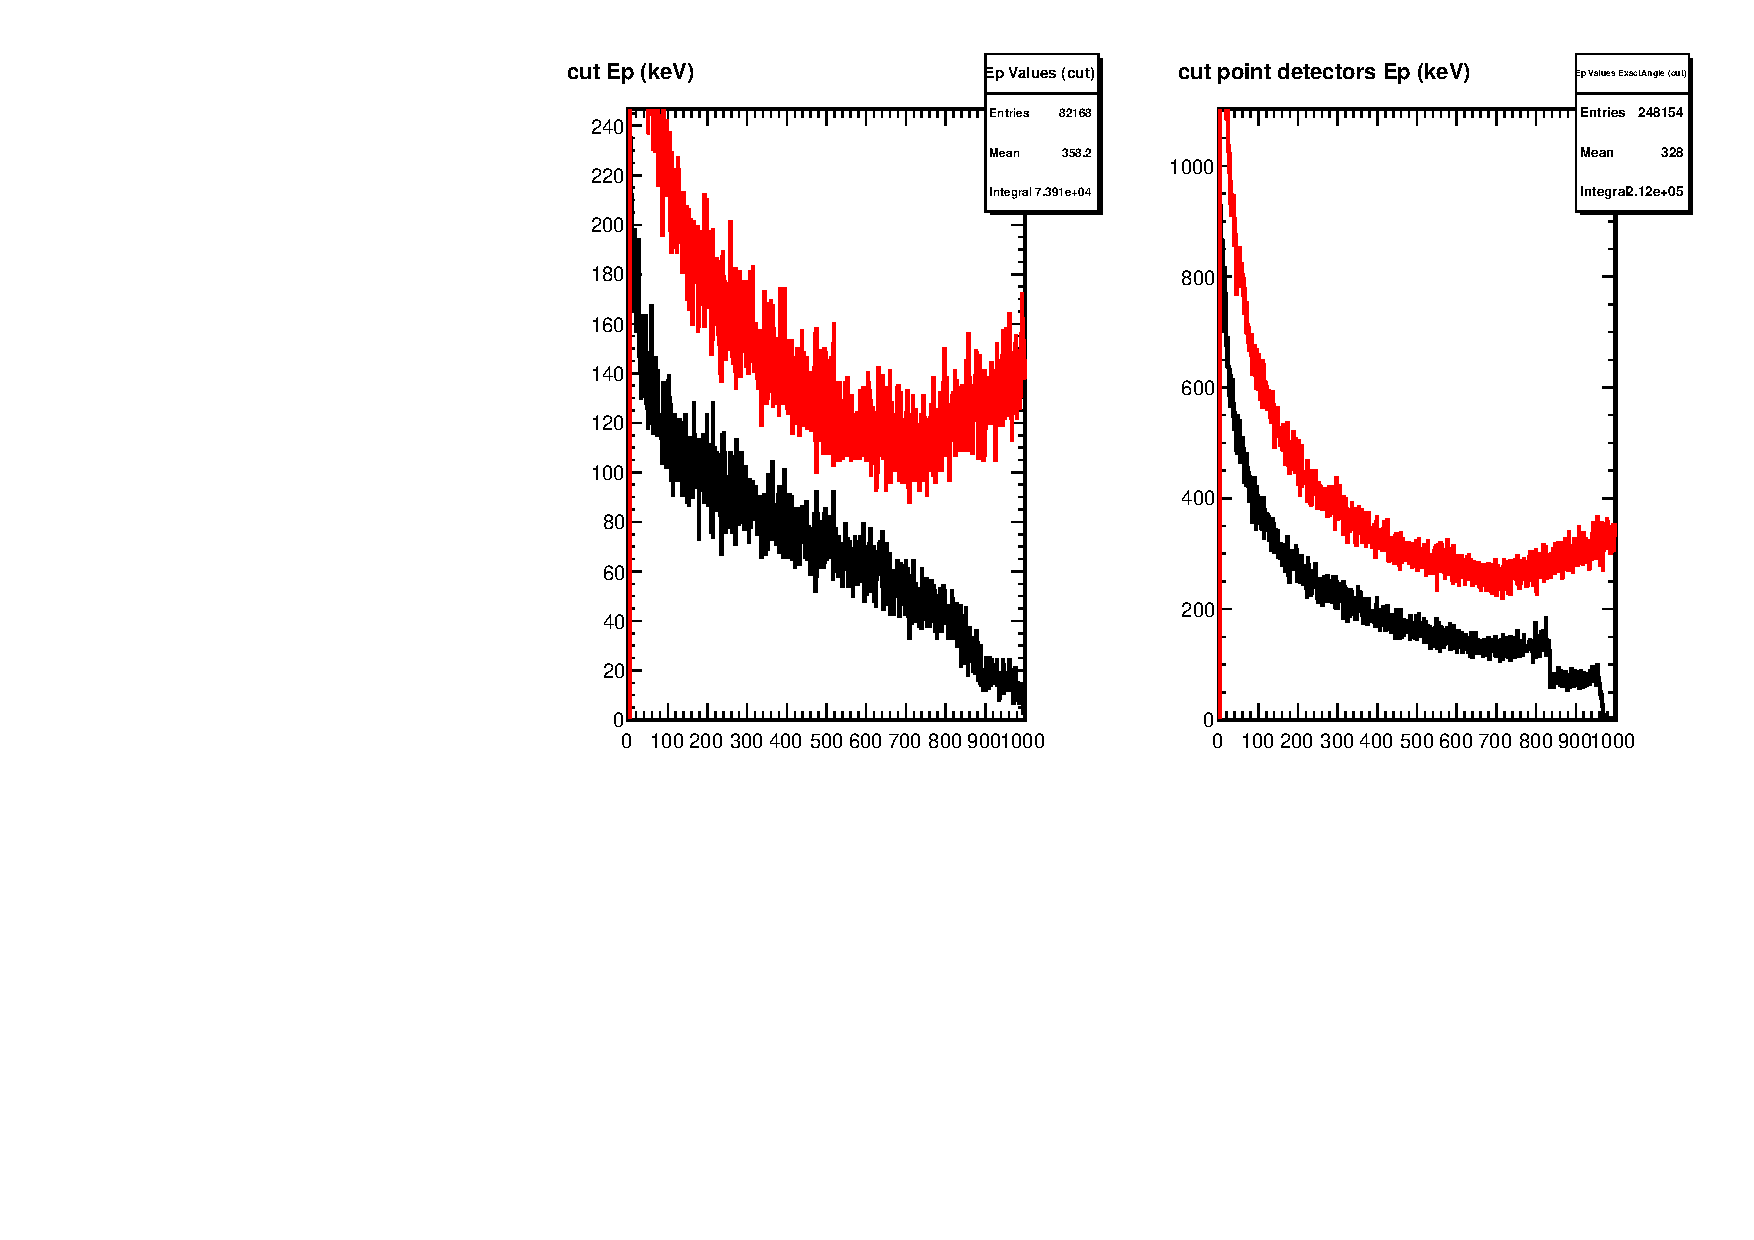
\includegraphics[width=\textwidth]{Ep}
  \caption{Proton energies calculated from E$_{\alpha 1}$ and
    E$_{\alpha 2}$. On left are the realistic models, and on the right
    are the ideal point detectors. Red lines correspond to uncut
    spectra (i.e., including high spectator momenta), and black is the
    cut (i.e., corresponding to the events in Fig.\ \ref{fig:2D}).}
  \label{fig:Ep}
\end{figure}

\begin{itemize}
\item No cross-sections have been included here, it's just to
  investigate solid angle effects.
\item For ideal, point-like models
  \begin{itemize}
  \item Alphas emitted at +- 45 deg exactly.
  \item Beamspot is a single point
  \item No target effects included
  \end{itemize}
\item Collimators are:
  \begin{itemize}
  \item Silicon: 1.1 mm
  \item Splitpole: 2 mm
  \end{itemize}
\item E$_{\alpha1}$ is measured in the silicon
\item Cut is an approximation to pick only small spectator momenta
\item Note:
  \begin{itemize}
  \item The steep rise in the number of counts for $\alpha$-pairs
    corresponding to low proton energy. This probably needs to be
    accounted for.
  \end{itemize}

\end{itemize}




\end{document}
